\section{Origem e Elementos Clássicos}

\begin{frame}[plain]
  \centering
  \Huge \insertsection
\end{frame}

\begin{frame}{A Origem da Teoria dos Grafos}
  \centering

  \begin{itemize}
    \item Surgiu com Leonhard Euler no século XVIII.
    \item Motivada pelo problema das \textbf{Pontes de Königsberg}.
  \end{itemize}
  
  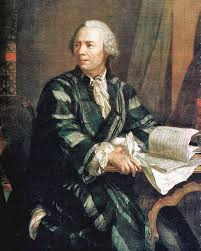
\includegraphics[width=0.5\textwidth]{./images/euler.jpeg}
\end{frame}

\begin{frame}{Uma Caminhada por Königsberg}
  \begin{itemize}
    \item O desafio: atravessar todas as pontes uma única vez.
    \item Euler provou que não era possível, iniciando a Teoria dos Grafos.
  \end{itemize}
  
  \centering
  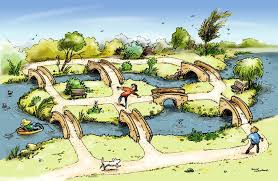
\includegraphics[width=0.5\textwidth]{./images/kpath.jpeg}

\end{frame}

\begin{frame}{Caminhos, Ciclos e Trajetos}
  \begin{itemize}
    \item \textbf{Caminho:} sequência de vértices adjacentes distintos.
    \item \textbf{Trilha:} sequência onde arestas não se repetem.
    \item \textbf{Circuito:} caminho fechado.
    \item \textbf{Ciclo:} circuito com vértices distintos (exceto o início/fim).
    \item \textbf{Trilha de Euler / Circuito de Euler}
  \end{itemize}
\end{frame}

\begin{frame}{Caminho}
  \centering
  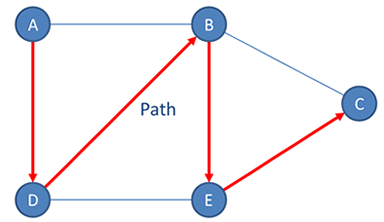
\includegraphics[width=1\textwidth\centering]{./images/path.png}
\end{frame}

\begin{frame}{Ciclo}
  \centering
  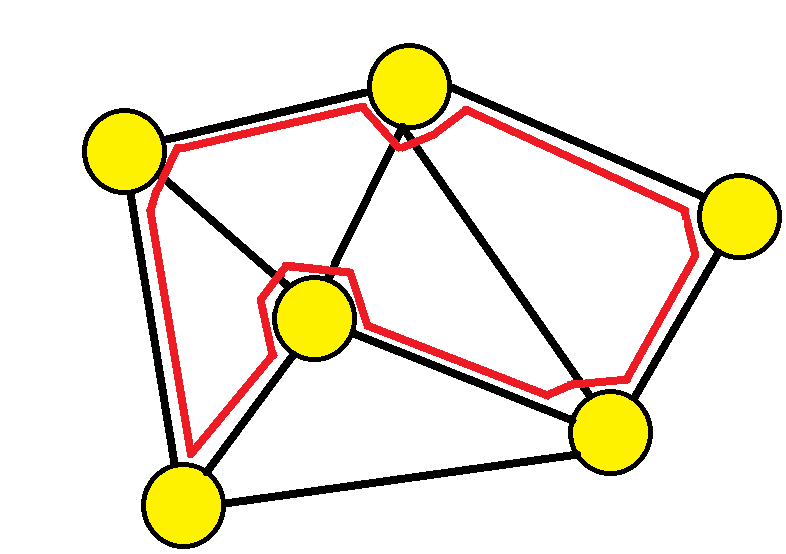
\includegraphics[width=1\textwidth\centering]{./images/circuit.png}
\end{frame}

\begin{frame}{Trilha de Euler}
  \centering
  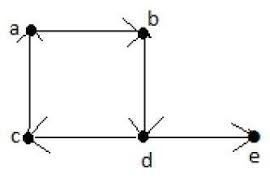
\includegraphics[width=0.5\textwidth\centering]{./images/eulerp.jpeg}
\end{frame}

\begin{frame}{Circuito de Euler}
  \centering
  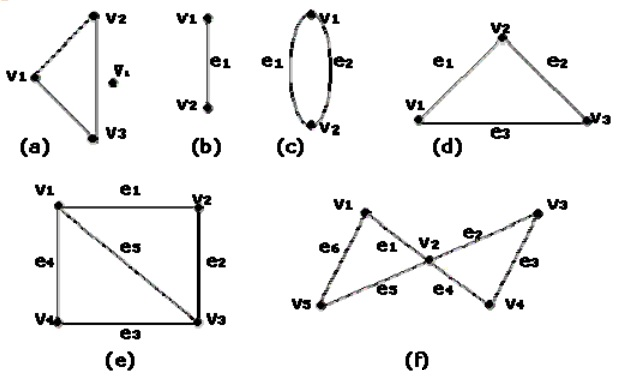
\includegraphics[width=0.75\textwidth\centering]{./images/eulerc.jpg}
\end{frame}

\begin{frame}{Teoremas de Euler}
  \begin{itemize}
    \item Um grafo possui um circuito de Euler se todos os vértices têm grau par.
    \item Possui uma trilha de Euler se exatamente dois vértices têm grau ímpar.
  \end{itemize}
\end{frame}

